\documentclass[tikz,border=15pt]{standalone}
\usepackage{tikz}
\usepackage{amsmath}
\usepackage{amssymb}
\usetikzlibrary{positioning, arrows.meta, calc, backgrounds, fit, shapes.geometric}

\colorlet{color_intent}{blue!60!black}
\colorlet{color_slot}{green!50!black}
\colorlet{color_topic}{red!60!black}
\colorlet{color_shared}{black!70}

\begin{document}

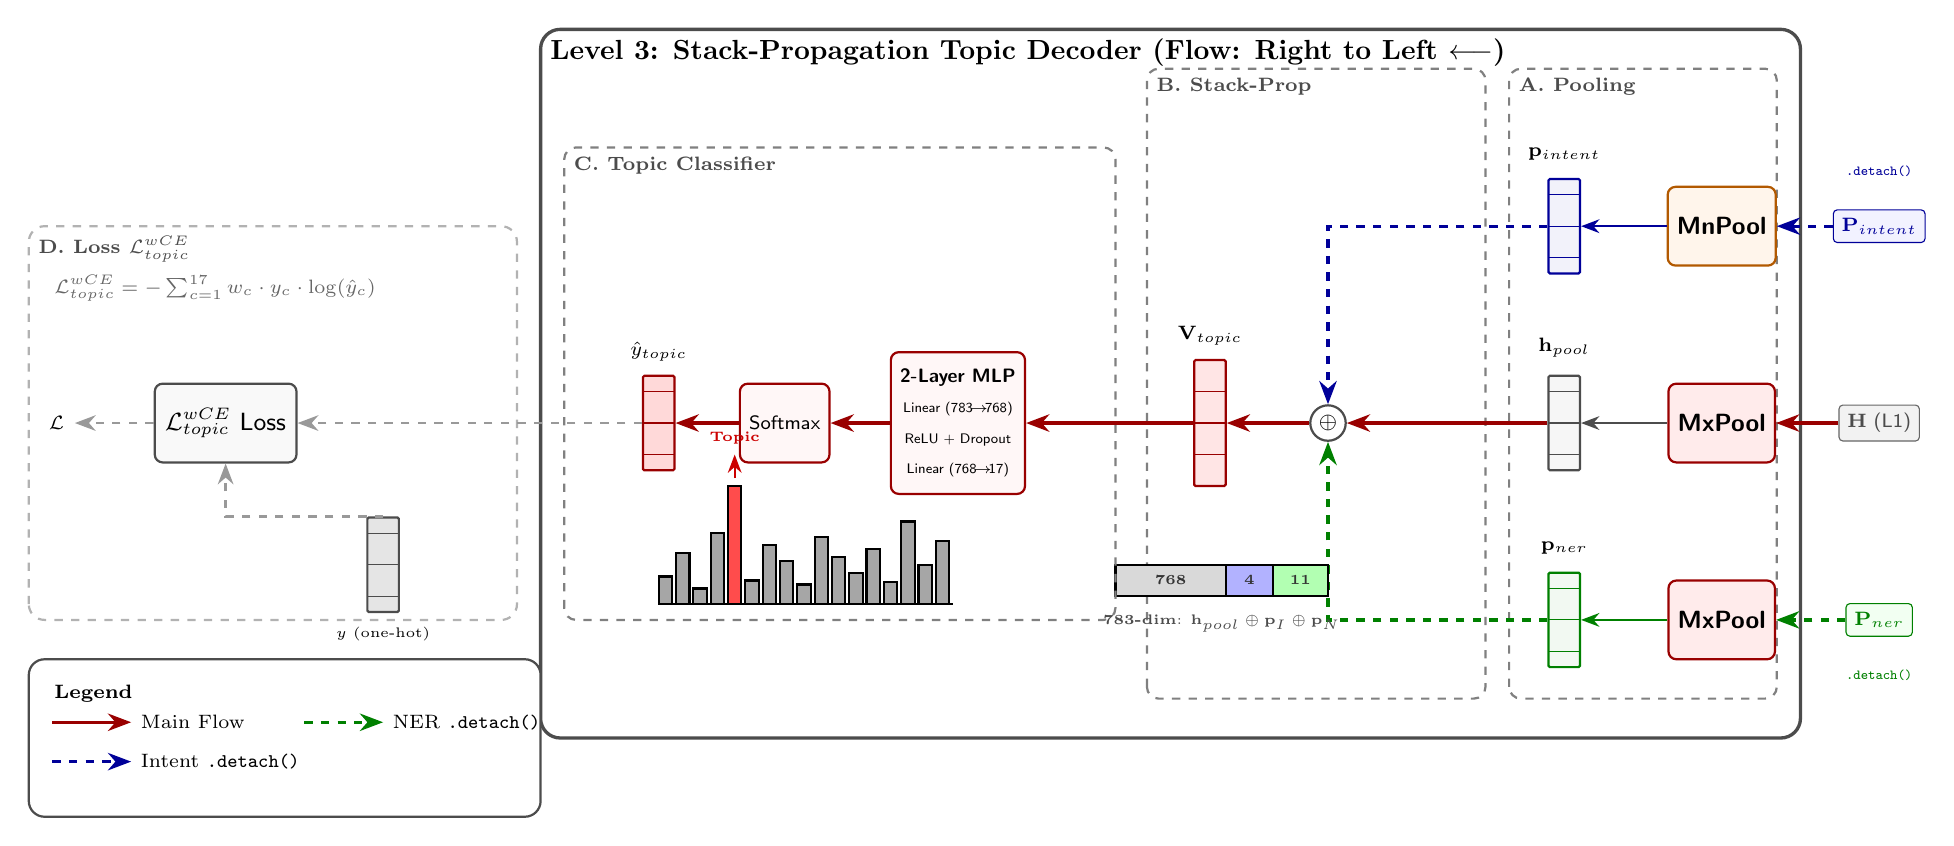
\begin{tikzpicture}[
    >=Stealth, font=\small\sffamily,
    mainbox/.style={draw=black!70, rounded corners=2.5mm, line width=1.2pt},
    subbox/.style={draw=black!50, dashed, rounded corners=1.5mm, line width=0.8pt},
    trainbox/.style={draw=black!30, dashed, rounded corners=2mm, line width=0.8pt},
    block/.style={draw=black!70, fill=white, rounded corners=1mm, thick, align=center},
    topic_block/.style={block, draw=red!60!black, fill=red!3},
    max_pool/.style={block, draw=red!60!black, fill=red!8, thick, minimum height=1cm},
    mean_pool/.style={block, draw=orange!70!black, fill=orange!8, thick, minimum height=1cm},
    op/.style={circle, draw=black!70, fill=white, inner sep=0.5pt, minimum size=0.45cm, thick, font=\footnotesize},
    arrow/.style={->, thick, draw=black!70},
    arrow_intent/.style={->, thick, draw=blue!60!black},
    arrow_slot/.style={->, thick, draw=green!50!black},
    link_solid/.style={->, line width=1.2pt, draw=red!60!black},
    link_dashed_blue/.style={->, line width=1.2pt, dashed, draw=blue!60!black},
    link_dashed_green/.style={->, line width=1.2pt, dashed, draw=green!50!black},
    link_dashed_gray/.style={->, line width=1.0pt, dashed, draw=gray!80},
    vector_grid/.style={
        draw=#1, thick, fill=#1!5, minimum width=0.4cm, minimum height=1.2cm, rounded corners=0.5pt,
        path picture={
            \foreach \y in {-0.4, 0, 0.4} \draw[#1, thin] (-0.2,\y) -- (0.2,\y);
        }
    }
]

%% ============================================================
%% TIER 3: STACK-PROPAGATION TOPIC DECODER
%% ============================================================
\draw[mainbox] (9.5, -13.0) rectangle (25.5, -4.0);
\node[anchor=north west, font=\bfseries] at (9.5, -4.0) {Level 3: Stack-Propagation Topic Decoder (Flow: Right to Left $\longleftarrow$)};

%% --- Inputs from Tier 2 (labeled entry points) ---
\node[font=\scriptsize\sffamily, text=color_intent, fill=blue!5, draw=blue!60!black,
      rounded corners=0.5mm, inner sep=3pt] (input_PI) at (26.5, -6.5) {$\mathbf{P}_{intent}$};
\node[font=\tiny\ttfamily, text=blue!60!black] at (26.5, -5.8) {.detach()};

\node[font=\scriptsize\sffamily, text=color_shared, fill=gray!10, draw=black!60,
      rounded corners=0.5mm, inner sep=3pt] (input_H) at (26.5, -9.0) {$\mathbf{H}$ (L1)};

\node[font=\scriptsize\sffamily, text=color_slot, fill=green!5, draw=green!50!black,
      rounded corners=0.5mm, inner sep=3pt] (input_PS) at (26.5, -11.5) {$\mathbf{P}_{ner}$};
\node[font=\tiny\ttfamily, text=green!50!black] at (26.5, -12.2) {.detach()};


%% --- A. Sentence-level Pooling ---
\draw[subbox] (21.8, -12.5) rectangle (25.2, -4.5);
\node[anchor=north west, font=\bfseries\scriptsize, text=black!70] at (21.8, -4.5) {A. Pooling};

\node[mean_pool] (l3_pool_I) at (24.5, -6.5) {\textbf{MnPool}};
\node[vector_grid=color_intent] (l3_vec_I) at (22.5, -6.5) {};
\node[above=0.1cm of l3_vec_I, font=\scriptsize] {$\mathbf{p}_{intent}$};
\draw[link_dashed_blue] (input_PI.west) -- (l3_pool_I.east);
\draw[arrow_intent] (l3_pool_I.west) -- (l3_vec_I.east);

\node[max_pool] (l3_pool_H) at (24.5, -9.0) {\textbf{MxPool}};
\node[vector_grid=color_shared] (l3_vec_H) at (22.5, -9.0) {};
\node[above=0.1cm of l3_vec_H, font=\scriptsize] {$\mathbf{h}_{pool}$};
\draw[link_solid] (input_H.west) -- (l3_pool_H.east);
\draw[arrow] (l3_pool_H.west) -- (l3_vec_H.east);

\node[max_pool] (l3_pool_S) at (24.5, -11.5) {\textbf{MxPool}};
\node[vector_grid=color_slot] (l3_vec_S) at (22.5, -11.5) {};
\node[above=0.1cm of l3_vec_S, font=\scriptsize] {$\mathbf{p}_{ner}$};
\draw[link_dashed_green] (input_PS.west) -- (l3_pool_S.east);
\draw[arrow_slot] (l3_pool_S.west) -- (l3_vec_S.east);


%% --- B. Stack-Propagation ---
\draw[subbox] (17.2, -12.5) rectangle (21.5, -4.5);
\node[anchor=north west, font=\bfseries\scriptsize, text=black!70] at (17.2, -4.5) {B. Stack-Prop};

\node[op] (l3_concat) at (19.5, -9.0) {$\oplus$};
\node[vector_grid=color_topic, fill=red!10, minimum height=1.6cm] (l3_vec_V) at (18.0, -9.0) {};
\node[above=0.05cm of l3_vec_V, font=\scriptsize] {$\mathbf{V}_{topic}$};

\draw[link_dashed_blue] (l3_vec_I.west) -| (19.5, -6.5) -- (l3_concat.north);
\draw[link_solid] (l3_vec_H.west) -- (l3_concat.east);
\draw[link_dashed_green] (l3_vec_S.west) -| (19.5, -11.5) -- (l3_concat.south);
\draw[link_solid] (l3_concat.west) -- (l3_vec_V.east);

% 783-dim bar: order matches code — cat([h_pool, intent, ner])
\begin{scope}[shift={(18.0, -11.0)}]
    \draw[fill=gray!30, thick] (-1.2, -0.2) rectangle (0.2, 0.2);
    \node[font=\tiny, text=black!80] at (-0.5, 0) {\textbf{768}};
    \draw[fill=blue!30, thick] (0.2, -0.2) rectangle (0.8, 0.2);
    \node[font=\tiny, text=black!80] at (0.5, 0) {\textbf{4}};
    \draw[fill=green!30, thick] (0.8, -0.2) rectangle (1.5, 0.2);
    \node[font=\tiny, text=black!80] at (1.15, 0) {\textbf{11}};
    \node[font=\tiny, align=center, text=black!70] at (0.15, -0.55)
        {\textbf{783-dim}: $\mathbf{h}_{pool} \oplus \mathbf{p}_I \oplus \mathbf{p}_N$};
\end{scope}


%% --- C. 2-Layer MLP Topic Classifier ---
\draw[subbox] (9.8, -11.5) rectangle (16.8, -5.5);
\node[anchor=north west, font=\bfseries\scriptsize, text=black!70] at (9.8, -5.5) {C. Topic Classifier};

\node[topic_block, minimum width=1.7cm, minimum height=1.8cm, align=center] (l3_lin_topic) at (14.8, -9.0) {
    \scriptsize \textbf{2-Layer MLP}\\
    \tiny Linear (783$\!\to\!$768)\\
    \tiny ReLU + Dropout\\
    \tiny Linear (768$\!\to\!$17)
};
\node[topic_block, minimum width=0.8cm, minimum height=1.0cm] (l3_soft_topic) at (12.6, -9.0) {\scriptsize Softmax};
\node[vector_grid=color_topic, fill=red!15] (l3_yhat) at (11.0, -9.0) {};
\node[above=0.05cm of l3_yhat, font=\scriptsize] {$\hat{y}_{topic}$};

\draw[link_solid] (l3_vec_V.west) -- (l3_lin_topic.east);
\draw[link_solid] (l3_lin_topic.west) -- (l3_soft_topic.east);
\draw[link_solid] (l3_soft_topic.west) -- (l3_yhat.east);

% Bar chart visualization
\begin{scope}[shift={(11.0, -11.3)}]
    \foreach \i/\h in {
        1/0.35, 2/0.65, 3/0.20, 4/0.90,
        5/1.50,
        6/0.30, 7/0.75, 8/0.55, 9/0.25,
        10/0.85, 11/0.60, 12/0.40, 13/0.70,
        14/0.28, 15/1.05, 16/0.50, 17/0.80
    } {
        \draw[fill=black!35, thick] (\i*0.22-0.22, 0) rectangle ++(0.17, \h);
    }
    \draw[fill=red!70, thick] (5*0.22-0.22, 0) rectangle ++(0.17, 1.50);
    \draw[->, thick, red!80!black] (5*0.22-0.135, 1.6) -- ++(0, 0.3)
        node[above, font=\tiny\bfseries, text=red!80!black] {Topic};
    \draw[thick] (0, 0) -- (17*0.22, 0);
\end{scope}


%% --- D. Weighted Cross-Entropy Loss ---
\draw[trainbox] (3.0, -11.5) rectangle (9.2, -6.5);
\node[anchor=north west, font=\bfseries\scriptsize, text=black!70] at (3.0, -6.5)
    {D. Loss $\mathcal{L}_{topic}^{wCE}$};

\node[block, minimum width=1.8cm, minimum height=1.0cm, fill=gray!5] (l3_loss) at (5.5, -9.0)
    {$\mathcal{L}_{topic}^{wCE}$ Loss};
\node[vector_grid=color_shared, fill=gray!20] (l3_y_true) at (7.5, -10.8) {};
\node[below=0.05cm of l3_y_true, font=\tiny] {$y$ (one-hot)};

\draw[link_dashed_gray] (l3_yhat.west) -- (l3_loss.east);
\draw[link_dashed_gray] (l3_y_true.north) -| (l3_loss.south);
\draw[link_dashed_gray] (l3_loss.west) -- ++(-1.0, 0) node[left, font=\bfseries\scriptsize] {$\mathcal{L}$};

%% --- Equation ---
\node[anchor=north west, font=\scriptsize, text=black!60, align=left] at (3.2, -7.0) {
    $\mathcal{L}_{topic}^{wCE} = -\sum_{c=1}^{17} w_c \cdot y_c \cdot \log(\hat{y}_c)$
};


%% ============================================================
%% LEGEND
%% ============================================================
\draw[draw=black!70, rounded corners=2mm, fill=white, thick] (3.0, -14.0) rectangle (9.5, -12.0);
\node[font=\bfseries\scriptsize, anchor=north west] at (3.2, -12.2) {Legend};

\draw[link_solid] (3.3, -12.8) -- (4.3, -12.8);
\node[anchor=west, font=\scriptsize] at (4.3, -12.8) {Main Flow};

\draw[link_dashed_blue] (3.3, -13.3) -- (4.3, -13.3);
\node[anchor=west, font=\scriptsize] at (4.3, -13.3) {Intent \texttt{.detach()}};

\draw[link_dashed_green] (6.5, -12.8) -- (7.5, -12.8);
\node[anchor=west, font=\scriptsize] at (7.5, -12.8) {NER \texttt{.detach()}};

\end{tikzpicture}

\end{document}
